% Ubah judul dan label berikut sesuai dengan yang diinginkan.
\section{Introduction}
\label{sec:pendahuluan}

% Ubah paragraf-paragraf pada bagian ini sesuai dengan yang diinginkan.

In the present age of digital technology, artificial intelligence has become intimately intertwined with several facets of human life. These advancements in technology have had a positive impact on various aspects of our lives. They have enhanced productivity by providing content recommendations on social media, virtual assistants, and spam filters. Additionally, they have improved efficiency through the implementation of intelligent transportation systems and automatic scheduling. Furthermore, they have contributed to entertainment and have played a significant role in the research and development sector of science and technology.
 
Diabetic retinopathy is a consequence of diabetes mellitus (DM) that occurs when blood vessels in the retina are damaged. The condition can result in diminished eyesight and potentially complete loss of vision \citet{Yusran2022}.

Diabetic retinopathy is a complication of diabetes mellitus that affects the eye. Clinically, diabetic retinopathy is defined as the presence of typical retinal microvascular signs in a person with diabetes mellitus. Vision loss develops from sequelae of maculopathy (macular edema and ischemia) and neovascularization of the retina (vitreous hemorrhage and retinal detachment) and iris (neovascular glaucoma) \citet{Cheung2010}. 
This is due to damage to the blood vessels in the retina, the light-sensitive layer of tissue at the back of the eye. Diabetic retinopathy is the leading cause of blindness in the working-age population in many countries \citet{fong2004diabetic}.

The condition was first observed by Eduard Jaeger in 1856 in his Journal entitled “Beitrage zur Pathologie des Auges” \citet{jaeger1855}. Further well-documented data proving a causal relationship between diabetes and maculopathy only appeared in 1869, when Henry Noyes published his report in the United States entitled “Retinitis in Glycosuria.” Noyes' observations were confirmed a few years later, in 1872, by Edward Nettleship in London, who further developed this topic in his paper entitled “On Edema or Cystic Diseases of the Retina.” \citet{Wolfensberger2001}.

Diabetic retinopathy can be classified into two main stages:

\begin{enumerate}
    \item \textbf{Non-Proliferative Diabetic Retinopathy (NPDR):} In this stage, the walls of the blood vessels in the retina are weakened. Microaneurysms may occur, leading to leakage of fluid and blood into the retina. This can result in macular swelling (macular edema) and vision loss \citet{aiello1998diabetic}.
    \item \textbf{Proliferative Diabetic Retinopathy (PDR):} Is an advanced stage of diabetic retinopathy. In RDP, abnormal new blood vessels begin to grow in the retina. These new blood vessels are fragile and can bleed into the vitreous, causing significant vision loss or even blindness \citet{king1998diabetes}.
\end{enumerate}

\begin{figure}[hbtp] \centering
    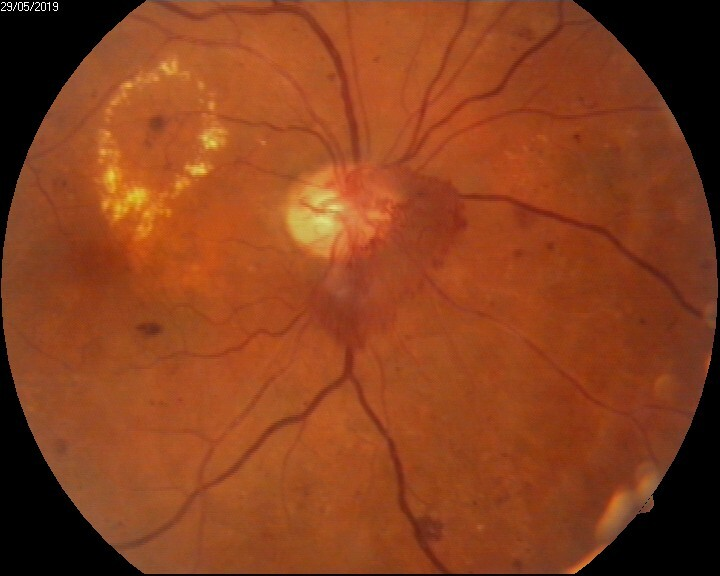
\includegraphics[width=0.4\textwidth]{gambar/PDR figure.jpg}
	% Keterangan gambar yang diinputkan
	\caption{Neovascularisation of Disc in Proliferative Diabetic Retinopathy \citet{Shukla2023-tq}}
	% Label referensi dari gambar yang diinputkan
	\label{fig:gambarPDR}
\end{figure}

Approximately 9.3 million individuals worldwide are afflicted with blindness caused by diabetic retinopathy, as reported by the World Health Organization (WHO). The projected figure is anticipated to rise to 12.6 million by the year 2040.

Early detection of diabetic retinopathy is essential in order to avoid the advancement of the illness and minimize the likelihood of severe consequences. Technology, particularly in the field of medical image processing, is now essential in the medical industry to enhance the early diagnosis of diabetic retinopathy. The Residual Neural Network (ResNet) is a well-established approach with numerous tools available for in-depth study.

ResNet is a neural network specifically created to tackle the issue of declining performance in neural networks with more depth. The residual technique enables ResNet to effectively optimize network learning on intricate data, such as medical images. The objective of this study is to examine diabetic retinopathy using a Convolutional Artificial Neural Network. 

This paper commences with a presentation of other research (Section \ref{sec:relatedresearch}).
This is followed by an explanation of the system architecture (Section \ref{sec:architecture}).
Based on the aforementioned findings, we present the results obtained in (Section \ref{sec:results}).
Finally, we present our conclusions based on the research conducted (Section \ref{sec:conclusion}).